% arara: pdflatex
% arara: pdflatex
\documentclass[journal]{IEEEtran}
\usepackage{graphicx}
\usepackage{	array,
			cite,
			graphicx,
			mathtools
			}
\usepackage{soul}
\usepackage{/Users/aviatorblue/Documents/mcode}
\graphicspath{ {./images/} } % Graphics Path



\begin{document}

\title{Direct Sequence-Spread Spectrum}
\author{David M Houston\\
		Oregon Institute of Technology\\\\
		}
\date{April 21, 2015}

\maketitle

\begin{abstract}
This project explained the ideas encompassing Direct Sequence-Spread Spectrum as it relates to RF communication systems and a discussion of Code-Division Multiple Access (CDMA). This was done using mathematical models of physical systems to conceptualize complex ideas and bring them down to realistic outcomes and measurable outputs.
\end{abstract}

\section{Introduction}
Direct Sequence-Spread Spectrum is a communication type which takes a digital I/O signal of information and modulates it with a pseudorandom binary sequence~\cite{ECPS}. This allows it to go under a significant amount of noise without a loss of data transfer to the receiver due to the signal riding on a noise signal. This allows the user to transmit in a very noisy environment where the noise floor is far above the expected thermal noise floor, or the KTB, an allows encryption of the data which is very secure based on the repetition of the pseudo-binary random number (PN)~\cite{ECPS}. This form of communication can be used in combination with Bilateral Phase-Shift Keying (BPSK), CDMA, and frequency hopping and is utilized in GPS, Wifi, and various secure communication arrays. 

\section{Signal Creation}
Spread spectrum is first created by a PN and a data signal. The data signal is a string of character created into an array of 8 bit binary number combinations based on the ASCII value of the characters. This gives our signal length as well some complexity for accurate transition analysis. This is fed through an encoder which converts a signal bit into 16 bits of that same value. This is used for voting to reduce bit error. This signal has a frequency spectrum which matches the following graphs (see Figure~\ref{fig:dio}). Usually it is preferred that a digital I/O signal is modulated by a PN whose bit rate is much higher than the digital I/O signals bit rate. This PN signal has a frequency spectrum which is very noisy containing all of the frequencies, just like white noise (see Figure~\ref{fig:PN}).\\

\begin{figure}[h!]
\centering
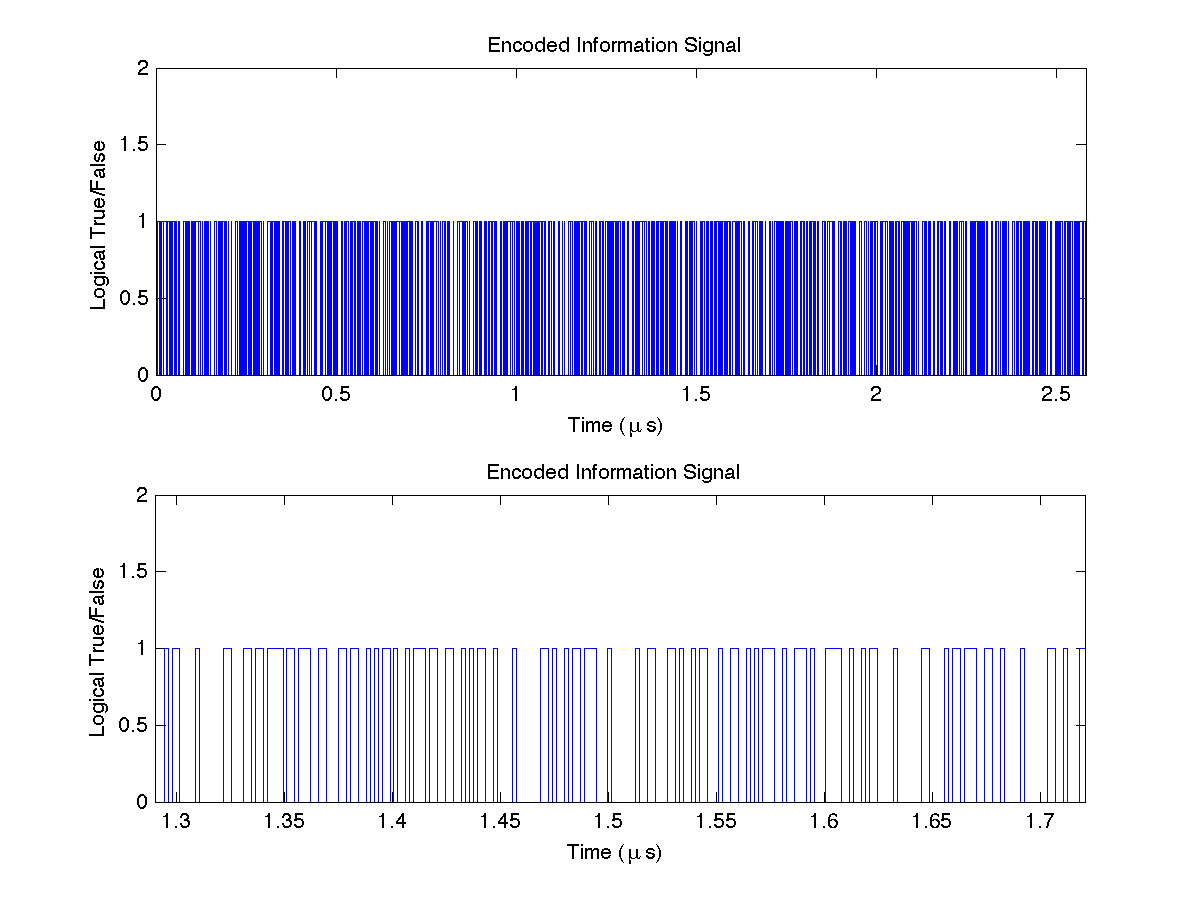
\includegraphics[width=3in]{encoded_signal.png}
\caption{Digital I/O Encoded Signal}
\label{fig:dio}
\end{figure}

\begin{figure}[h!]
\centering
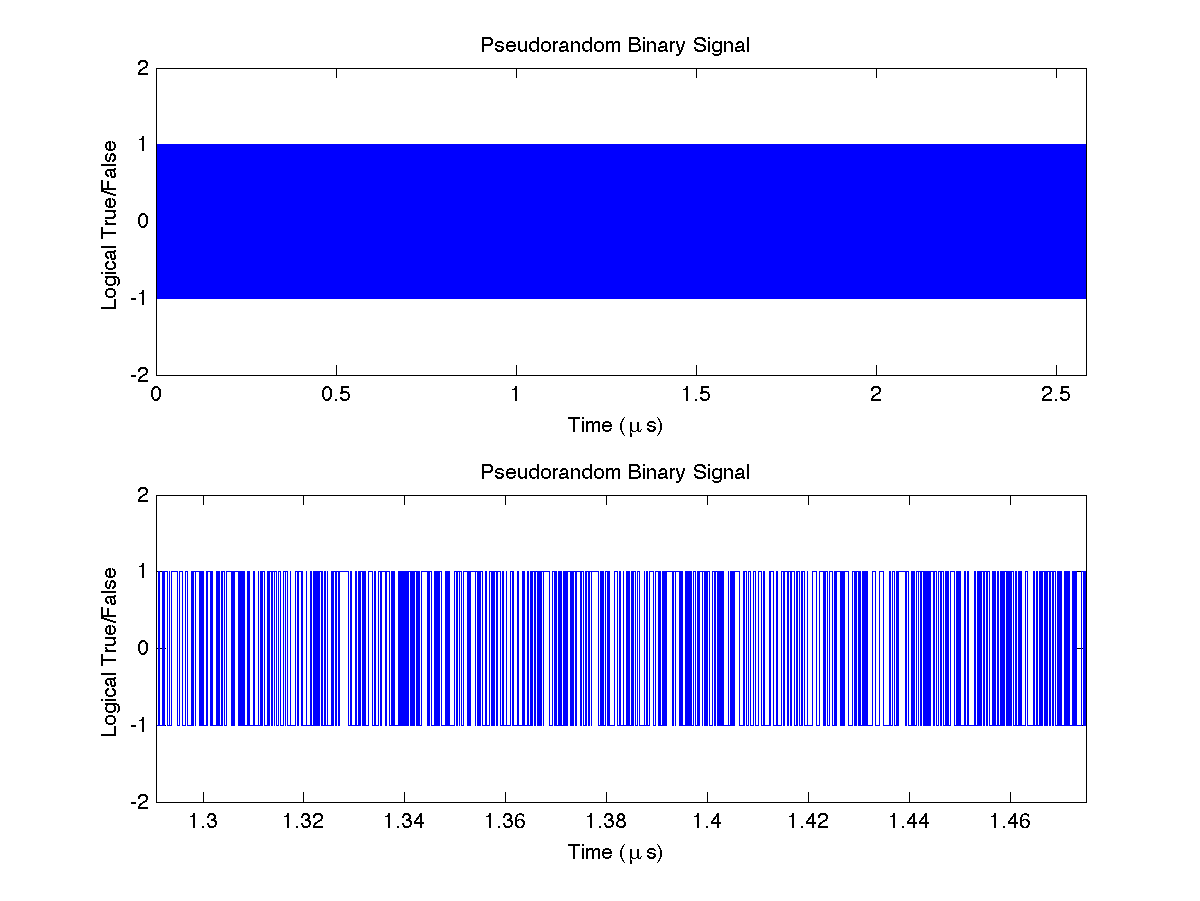
\includegraphics[width=3in]{pseudo_signal.png}
\caption{PN Signal}
\label{fig:PN}
\end{figure}
\end{appendices}

These two signals are then modulated together to form a digital I/O signal carried by a PN signal creating the basis for the DSSS signal (see Figure~\ref{fig:mod_PN}). This signal is then band limited and carrier by a large carrier signal (see Figure~\ref{fig:dsb_lc}) which can be demodulated by the receiver and then down converted. In order to reduce the bit transfer error of this form of communication the frequency of the PN was decreased to eliminate losses with the band limiting of the signal. When the signal was band limited a bit error of $\~13\%$ was observed. However, when the signal was transmitted on a carrier and then demodulated using a synchronous demodulator only a $3\%$ increase in bit loss was observed, after applying an amplifier to boost the signal.

\begin{figure}[h!]
\centering
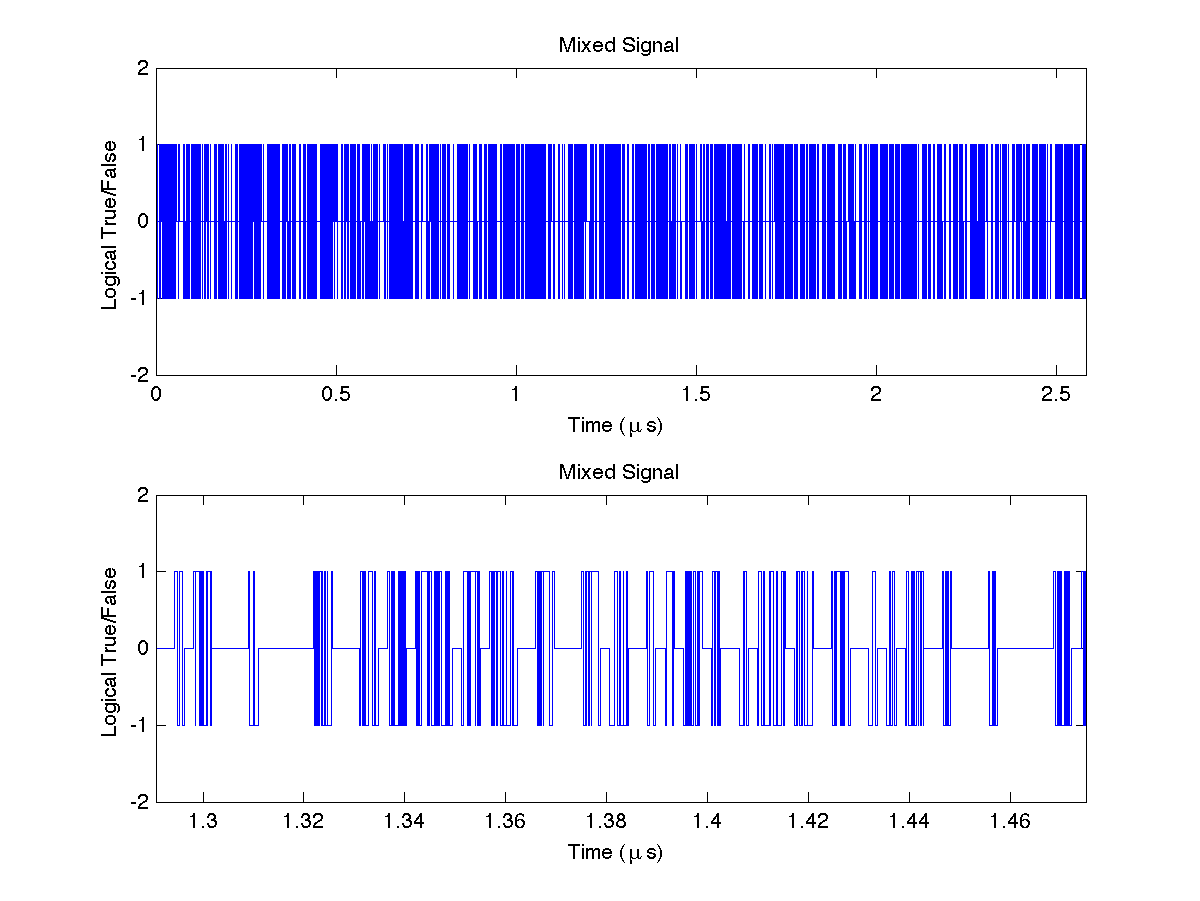
\includegraphics[width=3in]{dsss.png}
\caption{Modulated PN-Digital I/O Signal}
\label{fig:mod_PN}
\end{figure}

\begin{figure}[h!]
\centering
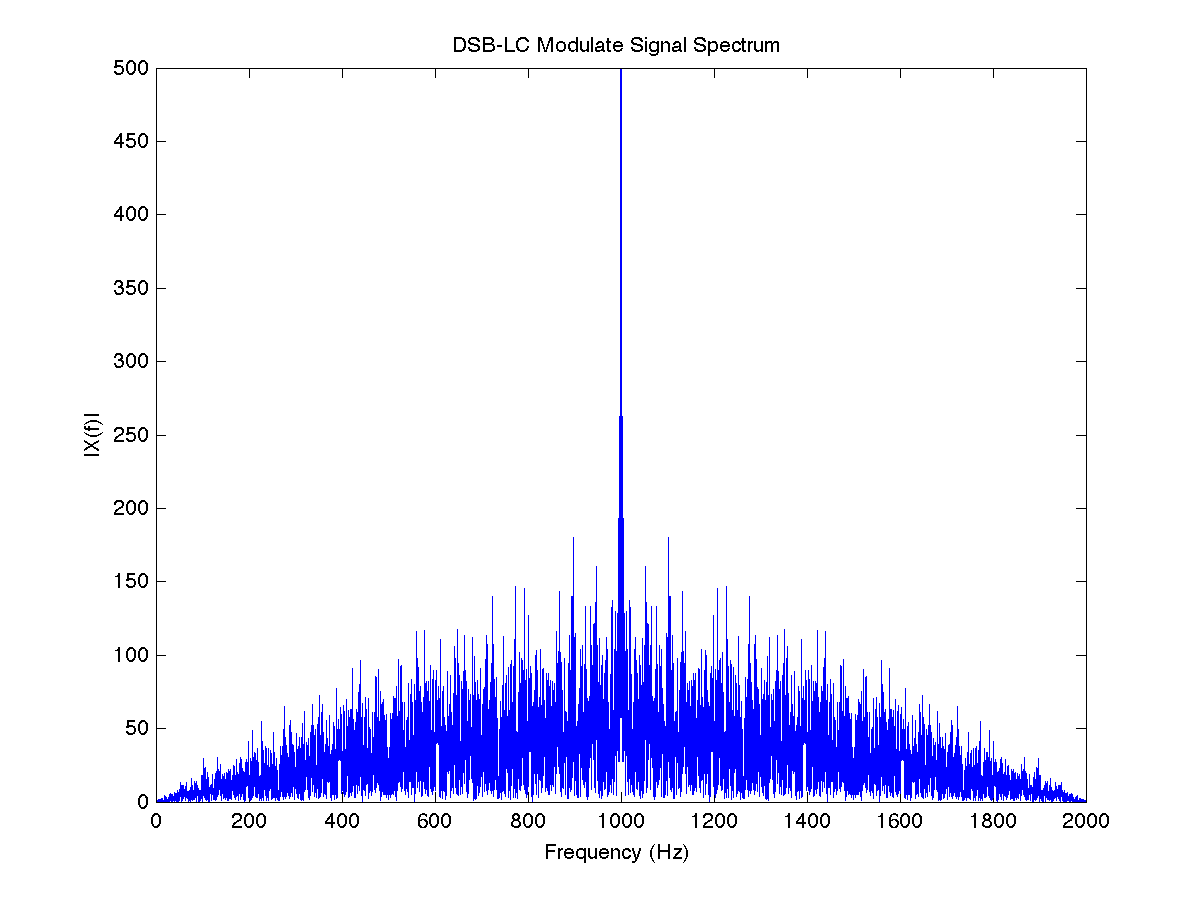
\includegraphics[width=3in]{mod_sig.png}
\caption{DSB-LC Signal}
\label{fig:dsb_lc}
\end{figure}

This signal is then despread to recreate the original signal. This despreading is done by multiplying the demodulating signal by the original PN (see Figure~\ref{fig:despread}). To verify the signals integrity a comparison was done to compare the bit error of the signal and it was found to have $\~16\%$ bit error. This error, as discussed above, is due to the band limiting of the signal for transmission.

\begin{figure}
\centering
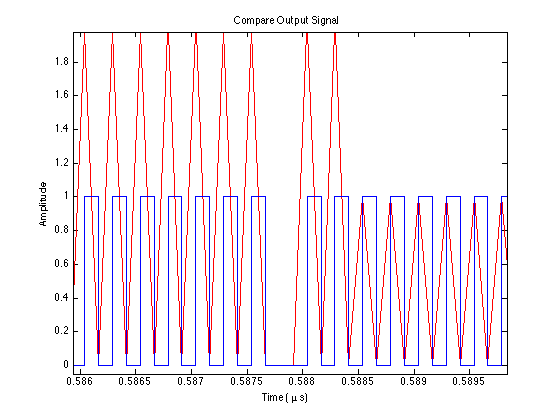
\includegraphics[width=3in]{despread.png}
\caption{Despread Signal Comparision}
\label{fig:despread}
\end{figure}

\section{White Noise}
When a signal accompanies additive white gaussian noise (AWGN) the signal to noise ratio decreases causing an increased error in the resulting signal. However, DSSS resilient to AWGN due to its modulation by a PN signal. The resilience of the DSSS signal can be seen in more detail by examining its frequency spectrum for the decreasing SNR (see Figure~\ref{fig:awgn_dsss}). 

\begin{figure}
\centering
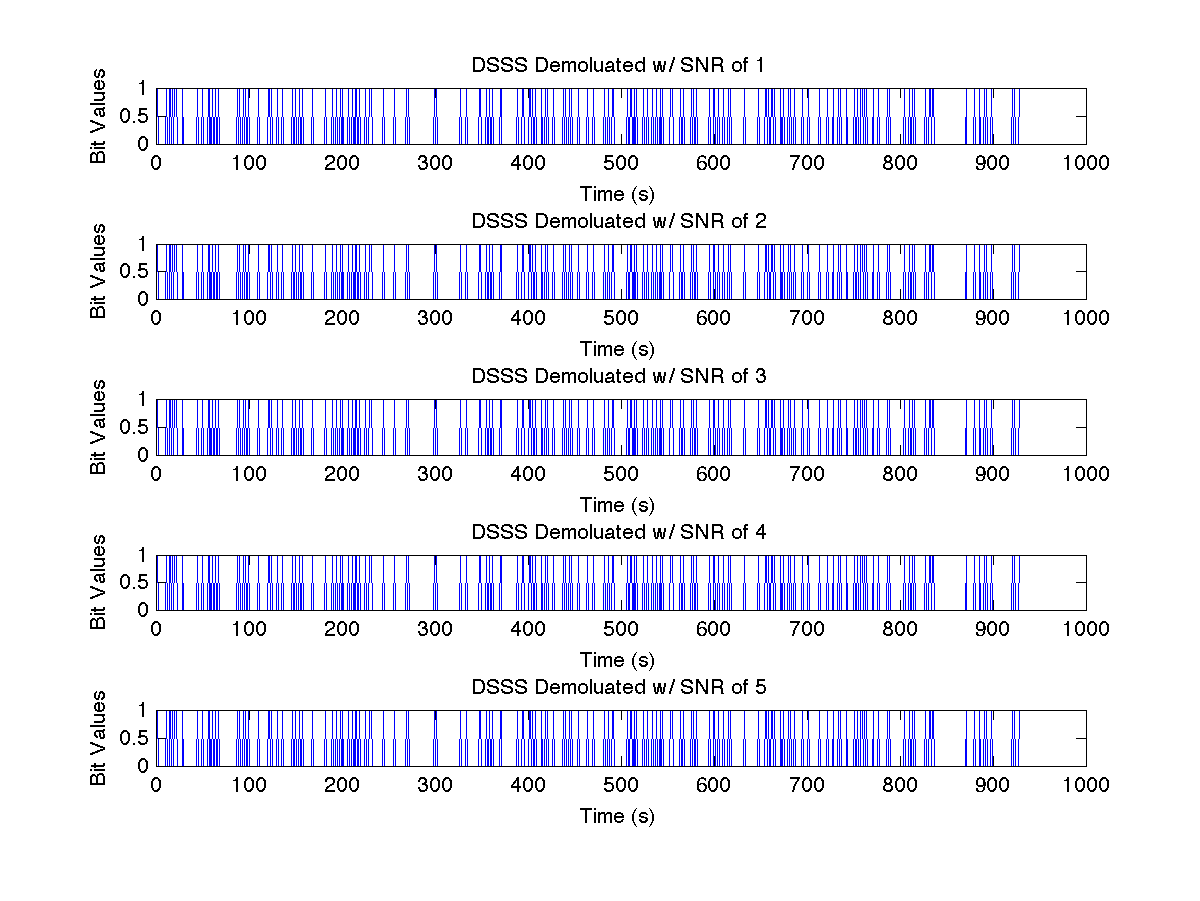
\includegraphics[width=3in]{awgn_dsss.png}
\caption{AWGN with DSSS Signal}
\label{fig:awgn_dsss}
\end{figure}

As the SNR decreases the bit error goes up, which makes sense. However for a signal to noise ratio of 0 dB a change in error is observed to be $\~3\%$. This is excellent considering the conditions that the signal is in. 

\section{Jamming}
Jamming is a process by which high power signals of specific frequencies are transmitted to "jam" or block a specific spectrum from allowing data transfer.  In the case of a typical DSB-LC AM signal, commonly used in Radio transmission, they can be very effective in destroying any chance of receiving data from the specific band you are looking on. However when jamming a DSSS signal the result is quite operational. For a jamming signal of white noise modulated at the same carrier frequency as the DSSS signal the increase in bit error is approximately $4\%$. This is the same effect the AWGN had on the signal which makes sense based on the nature of jamming.  

\begin{figure}
\centering
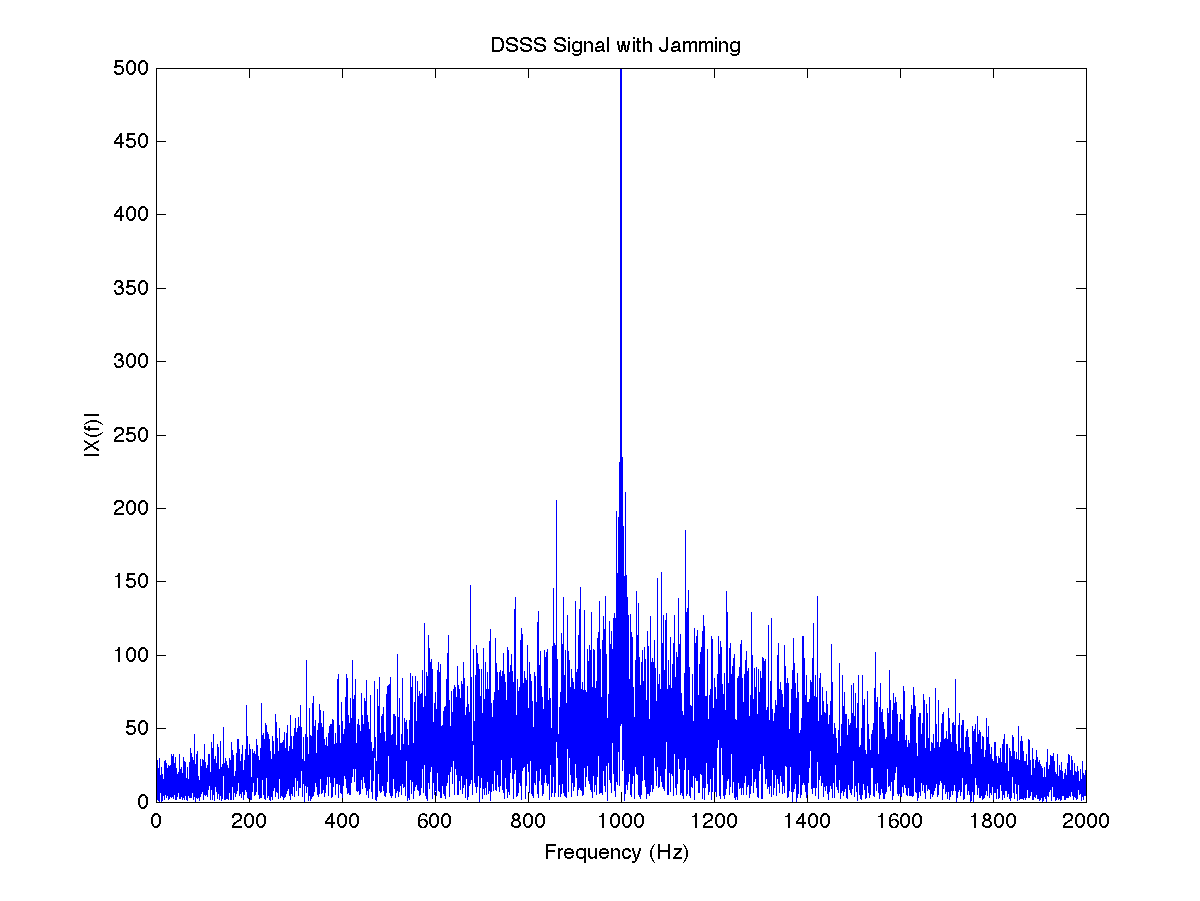
\includegraphics[width=3in]{jamming.png}
\caption{DSSS Signal w/ Jamming}
\label{fig:jamming}
\end{figure}

\section{CDMA}
The idea of having multiple users on the same frequency and spectrum has been around as long as telecommunications itself. The main idea behind CDMA is that you supply a list of users with their own device specific codes which are implemented in there transmitted signal and then used in the decoding of the data to determine where the data needs to go to~\cite{ECPS}. These codes would "modulate" the data signals and then autocorrelate with themselves in order to distinguish the data from one user to another. This could be implemented in DSSS by assigning each users a PN creating a very secure data transmission which would be almost undetectable unless the receiver had the key.

\section{Conclusion}
The results from using DSSS confirm its superiority over other forms of data transmission. This is due to its resilience against hostile jamming, its ability to transmit in very noisy conditions, and its ability and optimization for multiple access via CDMA.  

\begin{thebibliography}{1}

\bibitem{ECPS}
W.~D. Stanley and J.~M. Jeffords, \emph{Electronic Communication Principles and Systems}, 1st~ed.\hskip 1em plus
  0.5em minus 0.4em\relax USA: Delmar Cengage Learning, 2005.

\end{thebibliography}
\end{document}
